%Nearest neighbor problem
\section{Nearest neighbor problem}\label{nearestNeighborProblem}
	In this section we introduce the \nearestNeighborProblem, also known as nearest neighbor search (\nns).
	First, we define the problem. Then a short overview of related research is given, after which we elaborate on
	a solution called {\coverTree} \libref{coverTree}.
	\begin{mydef}
		Given a metric space $(M, d)$ (see \defref{metricSpace}) with $|M| \ge 2$ and a point $x \in M$,
		the \textnormal{nearest neighbor problem} asks for finding a point $y \in M$ such that
		\begin{align*}
			y = \argmin_{y' \in M \setminus \{x\}} d(x, y').
		\end{align*}
		The point $y$ is called \textnormal{nearest neighbor} of $x$.
	\end{mydef}
	% Nearest neighbor problem example
	\begin{figure}[!ht]
		 \begin{center}
			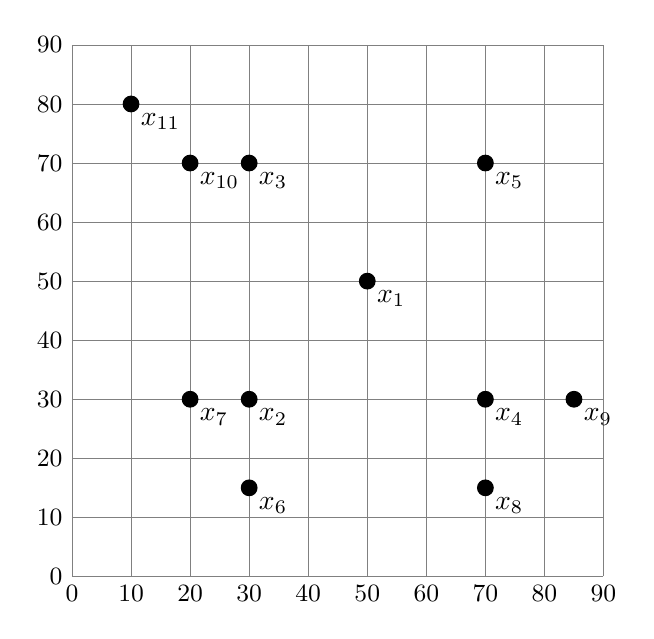
\begin{tikzpicture}[scale=0.75]
				% Grid
				\foreach \i [evaluate=\i as \ii using int(\i*10)] in {0,...,9} {
					\draw [very thin,gray] (\i,0) -- (\i,9)  node [below] at (\i,0) {\small{\color{black}{$\ii$}}};
					\draw [very thin,gray] (0,\i) -- (9,\i) node [left] at (0,\i) {\small{\color{black}{$\ii$}}};
				}
				
			 	% Nodes
			 	\node[inner sep=2pt, fill=black, circle, draw] (x1) at (5,5) {};
			 	\node[below right] at (x1) {$x_1$};
			 	
			 	\node[inner sep=2pt, fill=black, circle, draw] (x2) at (3,3) {};
			 	\node[below right] at (x2) {$x_2$};
			 	
			 	\node[inner sep=2pt, fill=black, circle, draw] (x3) at (3,7) {};
			 	\node[below right] at (x3) {$x_3$};
			 	
			 	\node[inner sep=2pt, fill=black, circle, draw] (x4) at (7,3) {};
			 	\node[below right] at (x4) {$x_4$};
			 	
			 	\node[inner sep=2pt, fill=black, circle, draw] (x5) at (7,7) {};
			 	\node[below right] at (x5) {$x_5$};
			 	
			 	\node[inner sep=2pt, fill=black, circle, draw] (x6) at (3,1.5) {};
			 	\node[below right] at (x6) {$x_6$};
			 	
			 	\node[inner sep=2pt, fill=black, circle, draw] (x7) at (2,3) {};
			 	\node[below right] at (x7) {$x_7$};
			 	
			 	\node[inner sep=2pt, fill=black, circle, draw] (x8) at (7,1.5) {};
			 	\node[below right] at (x8) {$x_8$};
			 	
			 	\node[inner sep=2pt, fill=black, circle, draw] (x9) at (8.5,3) {};
			 	\node[below right] at (x9) {$x_9$};
			 	
			 	\node[inner sep=2pt, fill=black, circle, draw] (x10) at (2,7) {};
			 	\node[below right] at (x10) {$x_{10}$};
			 	
			 	\node[inner sep=2pt, fill=black, circle, draw] (x11) at (1,8) {};
			 	\node[below right] at (x11) {$x_{11}$};
			\end{tikzpicture}
		\end{center}
		\caption{Grid showing eleven points in the cartesian plane $\mathbb{R}^2$.}
		\label{nearestNeighborProblemExample}
	\end{figure}\quad\\
	For following examples the toy data set shown in \figref{nearestNeighborProblemExample} is introduced.
	It consists of the points
	\begin{align*}
		x_1		&= (50, 50),\\
		x_2		&= (30, 30),\\
		x_3		&= (30, 70),\\
		x_4		&= (70, 30),\\
		x_5		&= (70, 70),\\
		x_6		&= (30, 15),\\
		x_7		&= (20, 30),\\
		x_8		&= (70, 15),\\
		x_9		&= (85, 30),\\
		x_{10}	&= (20, 70),\\
		x_{11}	&= (10, 80).
	\end{align*}
	All points are elements of the cartesian plane $\mathbb{R}$. The euclidean distance $d$ is chosen as metric on this set.
	For two dimensions it can be defined as:
	\begin{align*}
		d: \mathbb{R}^2 \times \mathbb{R}^2, ((x_1, y_1), (x_2, y_2)) \mapsto \sqrt{(x_2 - x_1)^2 + (y_2 - y_1)^2}
	\end{align*}
	Informally $d$ computes the \textit{ordinary} straight-line distance between two points.\\\\
	The nearest neighbor of $x_5$ is $x_1$ as
	\begin{align*}
		d(x_5, x_1)	&= \sqrt{(50 - 70)^2 + (50 - 70)^2}\\
				&= \sqrt{800}
	\end{align*}
	is smaller than all other distances to $x_5$, like
	\begin{align*}
		d(x_5, x_4)	&= \sqrt{(70 - 70)^2 + (30 - 70)^2}\\
				&= \sqrt{1600}.
	\end{align*}
	On the other hand, $x_1$ has four smallest neighbors:
	\begin{align*}
		d(x_1, x_2) = d(x_1, x_3) = d(x_1, x_4) = d(x_1, x_5)
	\end{align*}
	Any of them is a valid solution to the nearest neighbor problem of $x_1$.\\\\
	The search for a nearest neighbor is a well understood problem \libref{nnsOld, nnsNew} and has many
	applications. Without restrictions, solving the problem on general metrics was proven to
	require $\Omega(n)$ time \libref{nnsOld}, where $n$ is the amount of points.
	
	Typical approaches divide the space into regions, exploiting properties of the metric space.
	Common examples include {\kdTree}s \libref{kdTree}, {\vpTree}s \libref{vpTree},
	{\bkTree}s \libref{bkTree} and {\coverTree}s \libref{coverTree}.\\\\
	The problem also has a lot of variants. We elaborate on two of them:
	\begin{mydef}
		The \textnormal{k-nearest neighbors} of a point $x \in M$ are the
		$k$ closest points $\{y_1, y_2, \ldots, y_k\} \subseteq M$ to $x$. That is
		\begin{align*}
			y_1	&= \argmin_{y' \in M \setminus \{x\}} d(x, y'),\\
			y_2	&= \argmin_{y' \in M \setminus \{x, y_1\}} d(x, y'),\\
				&\vdots\\
			y_k	&= \argmin_{y' \in M \setminus \{x, y_1, \ldots, y_{k - 1}\}} d(x, y').
		\end{align*}
	\end{mydef}
	\begin{mydef}
		The \textnormal{k-neighborhood} of a point $x \in M$ is the set
		\begin{align*}
			\{y \in M \setminus \{x\} | d(x, y) \le k\}.
		\end{align*}
	\end{mydef}

%Cover tree
\subsection{Cover tree}
	\begin{mydef}\label{coverTree}
		A \textnormal{cover tree} $T$ on a metric space $(M, d)$ is a leveled tree $(V, E)$.
		
		The root is placed at the greatest level, denoted by $i_{\vmax} \in \mathbb{Z}$.
		The level of a node $v \in V$ is
		\begin{align*}
			\lvl(v)	&= i_{\vmax} - \depth(v).
		\end{align*}
		The lowest level is denoted by $i_{\vmin}$.
		Every node $v \in V$ is associated with a point $m \in M$. We write $\assoc(v) = m$.
		Nodes of a certain level form a \textit{cover} of points in $M$. A cover for a level $i$ is defined as
		\begin{align*}
			C_i	&= \{m \in M | \exists v \in V : \lvl(v) = i \land \assoc(v) = m\}.
		\end{align*}
		
		The following properties must hold
		\begin{itemize}
			\item[1.] For a level $i$ there must not exist nodes which are associated with the same point $m \in M$:
				\begin{align*}
					\nexists v, v' \in V : i = \lvl(v) = \lvl(v') \land v \neq v' \land \assoc(v) = \assoc(v')
				\end{align*}
				So each point can at most appear once per level.
			\item[2.] $C_i \subset C_{i - 1}$. This ensures that, once a point was associated with a node in a
				level, it appears in all lower levels too.
			\item[3.] Points are covered by their parents:
				\begin{align*}
					\forall p \in C_{i - 1} \exists q \in C_{i}: d(p, q) < 2^i
				\end{align*}
				and the node $v_p$ with $\lvl(v_p) = i \land \assoc(v_p) = p$ is the parent of the node
				$v_q$ with $\lvl(v_q) = i - 1 \land \assoc(v_q) = q$.
			\item[4.] Points in a cover $C_i$ have a separation of at least $2^i$, i.e.
				\begin{align*}
					\forall p, q \in C_i : p \neq q \Rightarrow d(p, q) > 2^i.
				\end{align*}
		\end{itemize}
	\end{mydef}
	A cover tree \libref{coverTree} has interesting distance properties on its nodes which allows for
	efficient retrieval of nearest neighbors. The general approach is straightforward. Given a node $v$ in the
	tree placed at level $i$, we know that all nodes of the subtree rooted at $v$ are associated with points
	inside a distance of at most $2^i$. This means that, if we search for a nearest neighbor,
	and traverse to a node $v$ in the tree, all nodes underneath $v$ are relatively close to $v$. So, if we already have a
	candidate for a nearest neighbor, with distance of $d$ and $v$ is already further away than $d + 2^i$;
	$v$ and all nodes in its subtree can not improve the distance.
	% Cover tree example
	\begin{figure}[!ht]
		 \begin{center}
			\begin{tikzpicture}[y = -1cm]
				% Levels
			 	\draw[redArea] (-0.6, -0.6) rectangle (10.6, 0.6);
			 	\node[left] at (-1, 0) {level $6$};
			 	
			 	\draw[blueArea] (-0.6, 1.4) rectangle (10.6, 2.6);
			 	\node[left] at (-1, 2) {level $5$};
			 	
			 	\draw[greenArea] (-0.6, 3.4) rectangle (10.6, 4.6);
			 	\node[left] at (-1, 4) {level $4$};
			 	
			 	\draw[orangeArea] (-0.6, 5.4) rectangle (10.6, 6.6);
			 	\node[left] at (-1, 6) {level $3$};
			 	
			 	% Nodes
			 	% Level 6
			 	\node[minimum size=9mm, circle, draw, fill=red!30] (6-1) at (3, 0) {$x_1$};
			 				 	
			 	% Level 5
			 	\node[minimum size=9mm, circle, draw, fill=blue!30] (5-11) at (0, 2) {$x_{11}$};
			 	\node[minimum size=9mm, circle, draw, fill=blue!30] (5-1) at (5.5, 2) {$x_1$};
			 	
			 	% Level 4
			 	\node[minimum size=9mm, circle, draw, fill=darkgreen!30] (4-11) at (0, 4) {$x_{11}$};
			 	\node[minimum size=9mm, circle, draw, fill=darkgreen!30] (4-1) at (1, 4) {$x_1$};
			 	\node[minimum size=9mm, circle, draw, fill=darkgreen!30] (4-2) at (3, 4) {$x_2$};
			 	\node[minimum size=9mm, circle, draw, fill=darkgreen!30] (4-3) at (5.5, 4) {$x_3$};
			 	\node[minimum size=9mm, circle, draw, fill=darkgreen!30] (4-4) at (8, 4) {$x_4$};
			 	\node[minimum size=9mm, circle, draw, fill=darkgreen!30] (4-5) at (10, 4) {$x_5$};
			 	
			 	% Level 3
			 	\node[minimum size=9mm, circle, draw, fill=orange!30] (3-11) at (0, 6) {$x_{11}$};
			 	\node[minimum size=9mm, circle, draw, fill=orange!30] (3-1) at (1, 6) {$x_1$};
			 	\node[minimum size=9mm, circle, draw, fill=orange!30] (3-2) at (2, 6) {$x_2$};
			 	\node[minimum size=9mm, circle, draw, fill=orange!30] (3-6) at (3, 6) {$x_6$};
			 	\node[minimum size=9mm, circle, draw, fill=orange!30] (3-7) at (4, 6) {$x_7$};
			 	\node[minimum size=9mm, circle, draw, fill=orange!30] (3-3) at (5, 6) {$x_3$};
			 	\node[minimum size=9mm, circle, draw, fill=orange!30] (3-10) at (6, 6) {$x_{10}$};
			 	\node[minimum size=9mm, circle, draw, fill=orange!30] (3-4) at (7, 6) {$x_4$};
			 	\node[minimum size=9mm, circle, draw, fill=orange!30] (3-8) at (8, 6) {$x_8$};
			 	\node[minimum size=9mm, circle, draw, fill=orange!30] (3-9) at (9, 6) {$x_9$};
			 	\node[minimum size=9mm, circle, draw, fill=orange!30] (3-5) at (10, 6) {$x_5$};
			 	
			 	% Edges
			 	% Level 6 to Level 5
			 	\draw[thick, ->] (6-1) to (5-11);
			 	\draw[thick, ->] (6-1) to (5-1);
			 	
			 	% Level 5 to Level 4
			 	\draw[thick, ->] (5-11) to (4-11);
			 	\draw[thick, ->] (5-1) to (4-1);
			 	\draw[thick, ->] (5-1) to (4-2);
			 	\draw[thick, ->] (5-1) to (4-3);
			 	\draw[thick, ->] (5-1) to (4-4);
			 	\draw[thick, ->] (5-1) to (4-5);
			 	
			 	% Level 4 to Level 3
			 	\draw[thick, ->] (4-11) to (3-11);
			 	\draw[thick, ->] (4-1) to (3-1);
			 	\draw[thick, ->] (4-2) to (3-2);
			 	\draw[thick, ->] (4-2) to (3-6);
			 	\draw[thick, ->] (4-2) to (3-7);
			 	\draw[thick, ->] (4-3) to (3-3);
			 	\draw[thick, ->] (4-3) to (3-10);
			 	\draw[thick, ->] (4-4) to (3-4);
			 	\draw[thick, ->] (4-4) to (3-8);
			 	\draw[thick, ->] (4-4) to (3-9);
			 	\draw[thick, ->] (4-5) to (3-5);
			\end{tikzpicture}
		\end{center}
		\caption{Cover tree for the data set of \figref{nearestNeighborProblemExample}.
			Nodes are vertically grouped by their levels and highlighted accordingly.}
		\label{coverTreeExample}
	\end{figure}
	% Cover tree example range
	\begin{figure}[!ht]
		 \begin{center}
		 	% Level 6
			\begin{tikzpicture}[scale=0.6]
				% Grid
				\foreach \i [evaluate=\i as \ii using int(\i*10)] in {0,...,9} {
					\draw [very thin,gray] (\i,0) -- (\i,9);
					\draw [very thin,gray] (0,\i) -- (9,\i);
				}
				
			 	% Nodes
			 	\node[inner sep=2pt, fill=red, circle, draw] (x1) at (5,5) {};
			 	\node[below right] at (x1) {$x_1$};
			 	
			 	\node[inner sep=2pt, fill=black, circle, draw] (x2) at (3,3) {};
			 	\node[below right] at (x2) {$x_2$};
			 	
			 	\node[inner sep=2pt, fill=black, circle, draw] (x3) at (3,7) {};
			 	\node[below right] at (x3) {$x_3$};
			 	
			 	\node[inner sep=2pt, fill=black, circle, draw] (x4) at (7,3) {};
			 	\node[below right] at (x4) {$x_4$};
			 	
			 	\node[inner sep=2pt, fill=black, circle, draw] (x5) at (7,7) {};
			 	\node[below right] at (x5) {$x_5$};
			 	
			 	\node[inner sep=2pt, fill=black, circle, draw] (x6) at (3,1.5) {};
			 	\node[below right] at (x6) {$x_6$};
			 	
			 	\node[inner sep=2pt, fill=black, circle, draw] (x7) at (2,3) {};
			 	\node[below right] at (x7) {$x_7$};
			 	
			 	\node[inner sep=2pt, fill=black, circle, draw] (x8) at (7,1.5) {};
			 	\node[below right] at (x8) {$x_8$};
			 	
			 	\node[inner sep=2pt, fill=black, circle, draw] (x9) at (8.5,3) {};
			 	\node[below right] at (x9) {$x_9$};
			 	
			 	\node[inner sep=2pt, fill=black, circle, draw] (x10) at (2,7) {};
			 	\node[below right] at (x10) {$x_{10}$};
			 	
			 	\node[inner sep=2pt, fill=black, circle, draw] (x11) at (1,8) {};
			 	\node[below right] at (x11) {$x_{11}$};
			 	
			 	% Circles
			 	\draw[clip] (0, 0) rectangle (9, 9);
			 	\node[inner sep=77pt, circle, draw=red, opacity=0.5, pattern=north west lines, pattern color=red] at (x1) {};
			\end{tikzpicture}
			% Level 5
			\begin{tikzpicture}[scale=0.6]
				% Grid
				\foreach \i [evaluate=\i as \ii using int(\i*10)] in {0,...,9} {
					\draw [very thin,gray] (\i,0) -- (\i,9);
					\draw [very thin,gray] (0,\i) -- (9,\i);
				}
				
			 	% Nodes
			 	\node[inner sep=2pt, fill=blue, circle, draw] (x1) at (5,5) {};
			 	\node[below right] at (x1) {$x_1$};
			 	
			 	\node[inner sep=2pt, fill=black, circle, draw] (x2) at (3,3) {};
			 	\node[below right] at (x2) {$x_2$};
			 	
			 	\node[inner sep=2pt, fill=black, circle, draw] (x3) at (3,7) {};
			 	\node[below right] at (x3) {$x_3$};
			 	
			 	\node[inner sep=2pt, fill=black, circle, draw] (x4) at (7,3) {};
			 	\node[below right] at (x4) {$x_4$};
			 	
			 	\node[inner sep=2pt, fill=black, circle, draw] (x5) at (7,7) {};
			 	\node[below right] at (x5) {$x_5$};
			 	
			 	\node[inner sep=2pt, fill=black, circle, draw] (x6) at (3,1.5) {};
			 	\node[below right] at (x6) {$x_6$};
			 	
			 	\node[inner sep=2pt, fill=black, circle, draw] (x7) at (2,3) {};
			 	\node[below right] at (x7) {$x_7$};
			 	
			 	\node[inner sep=2pt, fill=black, circle, draw] (x8) at (7,1.5) {};
			 	\node[below right] at (x8) {$x_8$};
			 	
			 	\node[inner sep=2pt, fill=black, circle, draw] (x9) at (8.5,3) {};
			 	\node[below right] at (x9) {$x_9$};
			 	
			 	\node[inner sep=2pt, fill=black, circle, draw] (x10) at (2,7) {};
			 	\node[below right] at (x10) {$x_{10}$};
			 	
			 	\node[inner sep=2pt, fill=blue, circle, draw] (x11) at (1,8) {};
			 	\node[below right] at (x11) {$x_{11}$};
			 	
			 	% Circles
			 	\draw[clip] (0, 0) rectangle (9, 9);
			 	\node[inner sep=38pt, circle, draw=blue, opacity=0.5, pattern=dots, pattern color=blue] at (x1) {};
			 	\node[inner sep=38pt, circle, draw=blue, opacity=0.5, pattern=dots, pattern color=blue] at (x11) {};
			\end{tikzpicture}\\\phantom{v}\quad\\
			% Level 4
			\begin{tikzpicture}[scale=0.6]
				% Grid
				\foreach \i [evaluate=\i as \ii using int(\i*10)] in {0,...,9} {
					\draw [very thin,gray] (\i,0) -- (\i,9);
					\draw [very thin,gray] (0,\i) -- (9,\i);
				}
				
			 	% Nodes
			 	\node[inner sep=2pt, fill=darkgreen, circle, draw] (x1) at (5,5) {};
			 	\node[below right] at (x1) {$x_1$};
			 	
			 	\node[inner sep=2pt, fill=darkgreen, circle, draw] (x2) at (3,3) {};
			 	\node[below right] at (x2) {$x_2$};
			 	
			 	\node[inner sep=2pt, fill=darkgreen, circle, draw] (x3) at (3,7) {};
			 	\node[below right] at (x3) {$x_3$};
			 	
			 	\node[inner sep=2pt, fill=darkgreen, circle, draw] (x4) at (7,3) {};
			 	\node[below right] at (x4) {$x_4$};
			 	
			 	\node[inner sep=2pt, fill=darkgreen, circle, draw] (x5) at (7,7) {};
			 	\node[below right] at (x5) {$x_5$};
			 	
			 	\node[inner sep=2pt, fill=black, circle, draw] (x6) at (3,1.5) {};
			 	\node[below right] at (x6) {$x_6$};
			 	
			 	\node[inner sep=2pt, fill=black, circle, draw] (x7) at (2,3) {};
			 	\node[below right] at (x7) {$x_7$};
			 	
			 	\node[inner sep=2pt, fill=black, circle, draw] (x8) at (7,1.5) {};
			 	\node[below right] at (x8) {$x_8$};
			 	
			 	\node[inner sep=2pt, fill=black, circle, draw] (x9) at (8.5,3) {};
			 	\node[below right] at (x9) {$x_9$};
			 	
			 	\node[inner sep=2pt, fill=black, circle, draw] (x10) at (2,7) {};
			 	\node[below right] at (x10) {$x_{10}$};
			 	
			 	\node[inner sep=2pt, fill=darkgreen, circle, draw] (x11) at (1,8) {};
			 	\node[below right] at (x11) {$x_{11}$};
			 	
			 	% Circles
			 	\draw[clip] (0, 0) rectangle (9, 9);
			 	\node[inner sep=19pt, circle, draw=darkgreen, opacity=0.5, pattern=horizontal lines, pattern color=darkgreen] at (x1) {};
			 	\node[inner sep=19pt, circle, draw=darkgreen, opacity=0.5, pattern=horizontal lines, pattern color=darkgreen] at (x2) {};
			 	\node[inner sep=19pt, circle, draw=darkgreen, opacity=0.5, pattern=horizontal lines, pattern color=darkgreen] at (x3) {};
			 	\node[inner sep=19pt, circle, draw=darkgreen, opacity=0.5, pattern=horizontal lines, pattern color=darkgreen] at (x4) {};
			 	\node[inner sep=19pt, circle, draw=darkgreen, opacity=0.5, pattern=horizontal lines, pattern color=darkgreen] at (x5) {};
			 	\node[inner sep=19pt, circle, draw=darkgreen, opacity=0.5, pattern=horizontal lines, pattern color=darkgreen] at (x11) {};
			\end{tikzpicture}
			% Level 3
			\begin{tikzpicture}[scale=0.6]
				% Grid
				\foreach \i [evaluate=\i as \ii using int(\i*10)] in {0,...,9} {
					\draw [very thin,gray] (\i,0) -- (\i,9);
					\draw [very thin,gray] (0,\i) -- (9,\i);
				}
				
			 	% Nodes
			 	\node[inner sep=2pt, fill=orange, circle, draw] (x1) at (5,5) {};
			 	\node[below right] at (x1) {$x_1$};
			 	
			 	\node[inner sep=2pt, fill=orange, circle, draw] (x2) at (3,3) {};
			 	\node[below right] at (x2) {$x_2$};
			 	
			 	\node[inner sep=2pt, fill=orange, circle, draw] (x3) at (3,7) {};
			 	\node[below right] at (x3) {$x_3$};
			 	
			 	\node[inner sep=2pt, fill=orange, circle, draw] (x4) at (7,3) {};
			 	\node[below right] at (x4) {$x_4$};
			 	
			 	\node[inner sep=2pt, fill=orange, circle, draw] (x5) at (7,7) {};
			 	\node[below right] at (x5) {$x_5$};
			 	
			 	\node[inner sep=2pt, fill=orange, circle, draw] (x6) at (3,1.5) {};
			 	\node[below right] at (x6) {$x_6$};
			 	
			 	\node[inner sep=2pt, fill=orange, circle, draw] (x7) at (2,3) {};
			 	\node[below right] at (x7) {$x_7$};
			 	
			 	\node[inner sep=2pt, fill=orange, circle, draw] (x8) at (7,1.5) {};
			 	\node[below right] at (x8) {$x_8$};
			 	
			 	\node[inner sep=2pt, fill=orange, circle, draw] (x9) at (8.5,3) {};
			 	\node[below right] at (x9) {$x_9$};
			 	
			 	\node[inner sep=2pt, fill=orange, circle, draw] (x10) at (2,7) {};
			 	\node[below right] at (x10) {$x_{10}$};
			 	
			 	\node[inner sep=2pt, fill=orange, circle, draw] (x11) at (1,8) {};
			 	\node[below right] at (x11) {$x_{11}$};
			 	
			 	% Circles
			 	\draw[clip] (0, 0) rectangle (9, 9);
			 	\node[inner sep=10pt, circle, draw=orange, opacity=0.5, pattern=crosshatch, pattern color=orange] at (x1) {};
			 	\node[inner sep=10pt, circle, draw=orange, opacity=0.5, pattern=crosshatch, pattern color=orange] at (x2) {};
			 	\node[inner sep=10pt, circle, draw=orange, opacity=0.5, pattern=crosshatch, pattern color=orange] at (x3) {};
			 	\node[inner sep=10pt, circle, draw=orange, opacity=0.5, pattern=crosshatch, pattern color=orange] at (x4) {};
			 	\node[inner sep=10pt, circle, draw=orange, opacity=0.5, pattern=crosshatch, pattern color=orange] at (x5) {};
			 	\node[inner sep= 10pt, circle, draw=orange, opacity=0.5, pattern=crosshatch, pattern color=orange] at (x6) {};
			 	\node[inner sep=10pt, circle, draw=orange, opacity=0.5, pattern=crosshatch, pattern color=orange] at (x7) {};
			 	\node[inner sep=10pt, circle, draw=orange, opacity=0.5, pattern=crosshatch, pattern color=orange] at (x8) {};
			 	\node[inner sep=10pt, circle, draw=orange, opacity=0.5, pattern=crosshatch, pattern color=orange] at (x9) {};
			 	\node[inner sep=10pt, circle, draw=orange, opacity=0.5, pattern=crosshatch, pattern color=orange] at (x10) {};
			 	\node[inner sep=10pt, circle, draw=orange, opacity=0.5, pattern=crosshatch, pattern color=orange] at (x11) {};
			\end{tikzpicture}
		\end{center}
		\caption{Figure that shows the separation property for each level of the cover tree shown by \figref{coverTreeExample}.
			The levels are highlighted in the same manner than in the previous example. The levels are $6, 5, 4$ and $3$ from
			top left to bottom right. The radii around the points have a size of $2^6, 2^5, 2^4$ and $2^3$.}
		\label{coverTreeExampleRange}
	\end{figure}\quad\\
	\figref{coverTreeExample} shows a valid cover tree for the toy example illustrated by \figref{nearestNeighborProblemExample}.
	The covers are
	\begin{align*}
		C_6	&= \{x_1\},\\
		C_5	&= \{x_1, x_{11}\},\\
		C_4	&= \{x_1, x_2, x_3, x_4, x_5, x_{11}\},\\
		C_3	&= \{x_1, x_2, x_3, x_4, x_5, x_6, x_7, x_8, x_9, x_{10}, x_{11}\}.
	\end{align*}
	Clearly the first property holds, there is no level where a $x_i$ is associated with a node more than once.
	The second property holds too, it is
	\begin{align*}
		C_6 \subset C_5 \subset C_4 \subset C_3.
	\end{align*}
	For the last two properties we take a look at \figref{coverTreeExampleRange}. It illustrates the fourth property.
	The property states that all points in a cover $C_i$ must have a distance of at least $2^i$ to each other.
	For level $6$ this is trivial since the set only contains $x_1$. For level $5$ it must hold that
	\begin{align*}
		d(x_1, x_{11}) = 50 > 32 = 2^5,
	\end{align*}
	which is true. If this would not be the case, the figure would show the nodes included inside the circle
	around the other node. Analogously all nodes in $C_4$ and $C_3$ are separated enough from each other.\\\\
	The third property can easily be confirmed using the figure too. It states that a node in level $i - 1$ must
	be closer than $2^i$ to its parent. Obviously this holds for $x_1$ and $x_{11}$ in level $5$, as a radius
	of $2^6$ around their parent $x_1$ covers all nodes. Likewise are $x_1, x_2, x_3, x_4$ and $x_5$ included
	in the circle around their parent $x_1$ with radius $2^5$.
	
	Note that it is not necessary that a node covers its whole subtree in its level. As example, we refer to $x_1$ in level $5$
	which does not cover $x_{10}$, as $d(x_1, x_{10}) > 2^5$, though it is part of the subtree rooted at $x_1$. The third property only demands
	that a parent covers all its direct children, not grandchildren or similar.\\\\
	% Cover tree insertion
	\IncMargin{1em}
	\begin{algorithm}
		\SetKwInOut{Input}{input}
  		\SetKwInOut{Output}{output}
		\SetKwFunction{d}{d}\SetKwFunction{fchildren}{children}\SetKwFunction{insert}{insert}
		\BlankLine
		\Input{point $p \in M$, candidate cover set $Q_i \subseteq C_i$, level $i$}
		\Output{\true if $p$ was inserted at level $i - 1$, \false otherwise}
		\BlankLine
		$Q \leftarrow \{\fchildren(q) | q \in Q_i\}$\;
		\BlankLine
		\If{$d(p, Q) > 2^i$}{
			\Return \false\tcp*{Check separation}
		}\Else{
			$Q_{i - 1} \leftarrow \{q \in Q | \d(p, q) \le 2^i\}$\tcp*{Covering candidates}
			\BlankLine
			\If{$\neg\insert(p, Q_{i - 1}, i - 1) \land \d(p, Q_i) \le 2^i$}{
				pick any $q \in Q_{i} : \d(p, q) \le 2^i$\;
				append $q$ as child to $q$\;
				\Return \true\;
			}\Else{
				\Return \false\;
			}
		}
		\BlankLine
		\caption{Inserting a point into a cover tree operating on a metric space $(M, d)$.}\label{coverTreeInsert}
	\end{algorithm}\DecMargin{1em}\quad\\
	The cover tree is constructed using \algoref{coverTreeInsert} with the maximal level $i_{\vmax}$ and the cover
	set $C_k$ which only consists of the root. The algorithm is stated recursively, but can easily be implemented
	without recursion by descending the levels and only following relevant candidates.
	
	A point $p$ can be appended in level $i - 1$ to a parent $q$ in level $i$ if the point has enough separation to all other
	nodes in this level, meaning more than $2^{i - 1}$, and is covered by the parent, that is a distance of less than $2^i$.
	The algorithm searches such a point by descending the levels, computing the separation and appending it to a
	node if it also covers the point.\\\\
	% Cover tree nearest neighbor search
	\IncMargin{1em}
	\begin{algorithm}
		\SetKwInOut{Input}{input}
  		\SetKwInOut{Output}{output}
		\SetKwFunction{d}{d}\SetKwFunction{fchildren}{children}
		\BlankLine
		\Input{point $p \in M$}
		\Output{a nearest neighbor to $p$ in $M$}
		\BlankLine
		$Q_{i_{\vmax}} \leftarrow C_{i_{\vmax}}$\;
		\For{$i$ from $i_{\vmax}$ to $i_{\vmin}$}{
			$Q \leftarrow \{\fchildren(q) | q \in Q_i\}$\;
			$Q_{i - 1} \leftarrow \{q \in Q | \d(p, q) \le \d(p, Q) + 2^i\}$\;
		}
		$\Return \argmin_{q \in Q_{i_{\vmin}}} \d(p, q)$\;
		\BlankLine
		\caption{Searching a nearest neighbor in a cover tree operating on a metric space $(M, d)$.}\label{coverTreeSearch}
	\end{algorithm}\DecMargin{1em}\quad\\
	A search for a nearest neighbor follows a similar approach. \algoref{coverTreeSearch} starts at the root and traverses
	the tree by following the children. The candidate set is refined by only following children which are closer than
	\begin{align*}
		d(p, Q) + 2^i.
	\end{align*}
	There, the distance to the set represents the distance of the currently best candidate. Nodes in the subtree
	rooted at a child can maximally be $2^i$ closer than the child itself. Therefore, take a look
	at \figref{coverTreeExampleRange} where $x_2$ is maximally $2^5$ closer to $x_7$ than $x_1$, else it would not
	be covered by its parent $x_1$.
	Because of that the algorithm only follows children which can have nodes in their subtree
	that improve over the currently best candidate. Other children are rejected.
	
	Note that the algorithm must track down all levels, as another node could show up in the lowest level because of
	the separation property.\\\\
	% Cover tree k-nearest neighbor search
	\IncMargin{1em}
	\begin{algorithm}
		\SetKwInOut{Input}{input}
  		\SetKwInOut{Output}{output}
		\SetKwFunction{d}{d}\SetKwFunction{fchildren}{children}
		\BlankLine
		\Input{point $p \in M$, amount $k \in \mathbb{N}$}
		\Output{$k$-nearest neighbors to $p$ in $M$}
		\BlankLine
		$Q_{i_{\vmax}} \leftarrow C_{i_{\vmax}}$\;
		\For{$i$ from $i_{\vmax}$ to $i_{\vmin}$}{
			$Q \leftarrow \{\fchildren(q) | q \in Q_i\}$\;
			\BlankLine
			perform a $k$-partial sort of $Q$, ascending in $\d(p, q)$\;
			let $q'$ be the $k$-th element of $Q$\;
			\BlankLine
			$Q_{i - 1} \leftarrow \{q \in Q | \d(p, q) \le \d(p, q') + 2^i\}$\;
		}
		\BlankLine
		perform a $k$-partial sort of $Q_{i_{\vmin}}$, ascending in $\d(p, q)$\;
		\Return first $k$ elements of $Q_{i_{\vmin}}$\;
		\BlankLine
		\caption{Searching the $k$-nearest neighbors in a cover tree operating on a metric space $(M, d)$.}\label{coverTreeKSearch}
	\end{algorithm}\DecMargin{1em}\quad\\
	% Cover tree k-neighborhood computation
	\IncMargin{1em}
	\begin{algorithm}
		\SetKwInOut{Input}{input}
  		\SetKwInOut{Output}{output}
		\SetKwFunction{d}{d}\SetKwFunction{fchildren}{children}
		\BlankLine
		\Input{point $p \in M$, radius $k \in \mathbb{R}_{\ge 0}$}
		\Output{$k$-neighborhood of $p$ in $M$}
		\BlankLine
		$Q_{i_{\vmax}} \leftarrow C_{i_{\vmax}}$\;
		\For{$i$ from $i_{\vmax}$ to $i_{\vmin}$}{
			$Q \leftarrow \{\fchildren(q) | q \in Q_i\}$\;
			$Q_{i - 1} \leftarrow \{q \in Q | \d(p, q) \le k + 2^i\}$\;
		}
		$\Return \{q \in Q_{i_{\vmin}} | \d(p, q) \le k\}$\;
		\BlankLine
		\caption{Computing the $k$-neighborhood by using a cover tree which operates on a metric space $(M, d)$.}\label{coverTreeKNeighborhood}
	\end{algorithm}\DecMargin{1em}\quad\\
	The cover tree can also be used to efficiently compute the $k$-nearest neighbors or the $k$-neighborhood.
	In order to compute the $k$-nearest neighbors, \algoref{coverTreeKSearch} extends the range bound from the currently
	best candidate to the $k$-th best candidate. Likewise does \algoref{coverTreeKNeighborhood} extend the bound to
	the given range $k$ instead of involving candidate distances.\\\\
	For other operations and a detailed analysis of the cover tree, as well as its complexity and a comparison
	against other techniques, refer to \libref{coverTree}.